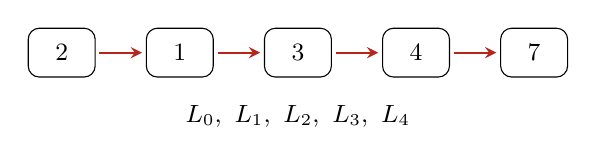
\begin{tikzpicture}[>=stealth,font=\small]
\foreach \x/\v in {0/2,1.5/1,3/3,4.5/4,6/7}{
\node[draw,rounded corners,minimum width=0.85cm,minimum height=.62cm] (n\x) at (\x,0) {$\v$};}
\foreach \a/\b in {0/1.5,1.5/3,3/4.5,4.5/6}{\draw[->,BrickRed,thick] (\a+.48,0)--(\b-.48,0);}
\node[below] at (3,-.55) {$L_0,\ L_1,\ L_2,\ L_3,\ L_4$};
\end{tikzpicture}
